\section{Method}
\label{sec:method}

In the following, we first introduce the mathematical formulation of the weakly-supervised 3D shape completion problem. Subsequently, we briefly discuss the concept of variational auto-encoders (\VAEs) \cite{Kingma2013ARXIV} which we use to learn a shape prior.
% -- which are used to learn a shape prior based on the reference shapes.
Finally, we formally derive our proposed amortized maximum likelihood (\AML) approach. The overall framework is also illustrated in Figure \ref{fig:method}.

\subsection{Problem Formulation}

In a supervised setting, our task can be described as follows: given a set of partial observations $\mathcal{X} = \{x_n\}_{n = 1}^N \subseteq \mathbb{R}^R$ and corresponding ground truth shapes $\mathcal{Y}^* = \{y_n^*\}_{n = 1}^N \subseteq \mathbb{R}^R$, learn a mapping $x_n \mapsto y_n^*$ that is able to generalize to previously unseen observations. Here, we assume $\mathbb{R}^R$ to be a suitable vector representation of observations and shapes; in practice, we resort to occupancy grids or signed distance functions (SDFs) defined on regular grids, \ie, $x_n, y_n^* \in \mathbb{R}^{H \times W \times D} \simeq \mathbb{R}^R$.
SDFs represent the distance of each voxel's center to the closest point on the surface; we use negative signs for interior voxels.
For the (partial) observations, we write $x_n \in \{0, 1, \uk\}^R$ to make missing information explicit; in particular, $x_{n,i} = \uk$ corresponds to unobserved voxels, while $x_{n,i} = 1$ and $x_{n,i} = 0$ correspond to occupied and unoccupied voxels, respectively.

On real data, \eg, KITTI \cite{Geiger2012CVPR}, supervised learning is often not possible as obtaining ground truth annotations is labor intensive (\eg, \cite{Menze2015CVPR,Xie2016CVPR}). Therefore, we target a weakly-supervised variant of the problem instead. Given observations $\mathcal{X}$ and a set of reference shapes $\mathcal{Y} = \{y_m\}_{m = 1}^M \subseteq \mathbb{R}^R$ both of the same, known object category, learn a mapping $x_n \mapsto \tilde{y}(x_n)$ such that the predicted shape $\tilde{y}(x_n)$ matches the unknown ground truth shape $y_n^*$ as close as possible.
Here, supervision is provided in the form of the known object category, allowing to derive the reference shapes from (watertight) triangular meshes; on real data, we also assume the object locations to be given in the form of 3D bounding boxes in order to extract the observations $\mathcal{X}$.
%\green{In practice, the reference shapes $\mathcal{Y}$ are derived from watertight, triangular meshes in order to obtain well-defined occupancy grids and SDFs.}
%In the following, we assume that the shapes $\mathcal{Y}$ are available as meshes from which we derive occupancy grids and SDFs; the observations are voxelized as described above.

\subsection{Shape Prior}
\label{subsec:method-prior}

We propose to use the provided reference shapes $\mathcal{Y}$ to learn a model of possible 3D shapes over the latent space $\mathcal{Z} = \mathbb{R}^Q$ with $Q \ll R$. The prior model is learned using a \VAE where the joint distribution $p(y, z)$ decomposes into $p(y, z) = p(y | z)p(z)$ with $p(z)$ being a unit Gaussian, \ie, $p(z) = \mathcal{N}(z;0, I_Q)$ with $I_Q \in \mathbb{R}^{R \times R}$ being the identity matrix. Sampling from the model is then performed by choosing $z \sim p(z)$ and subsequently sampling $y \sim p(y | z)$. For training the generative model, we also need to approximate the posterior $q(z | y) \approx p(z | y)$, \ie, the inference model. In the framework of the variational auto-encoder, both the so-called recognition model $q(z | y)$ and the generative model $p(y | z)$ -- corresponding to encoder and decoder -- are represented by neural networks. In particular,
\begin{align}
%\text{\bf Encoder: }
q(z | y) = \mathcal{N}(z_i; \mu_i(y), \text{diag}(\sigma_i^2(y)))
\end{align}
where $\mu(y), \sigma^2(y) \in \mathbb{R}^Q$ are predicted using the encoder neural network and $p(y_i | z)$ is assumed to be a Bernoulli distribution when working with occupancy grids, \ie, $p(y_i | z) = \text{Ber}(y_i ; \theta_i(z))$ while a Gaussian distribution is used when predicting SDFs, \ie, $p(y_i | z) = \mathcal{N}(y_i ; \mu_i(z), \sigma^2)$. In both cases, the parameters, \ie, $\theta_i(z)$ or $\mu_i(z)$, are predicted using the decoder neural network. For SDFs, we neglect the variance ($\sigma^2 = 1$) as it merely scales the training objective.

In the framework of variational inference, the parameters of the encoder and the decoder are found by maximizing the likelihood $p(y)$. In practice, the likelihood is often intractable. Instead, the evidence lower bound is maximized, resulting in the following loss to be minimized:
\begin{align}
\mathcal{L}_{\text{VAE}}(w) = - \mathbb{E}_{q(z |y)}[\ln p(y|z)] + \text{KL}(q(z | y)| p(z)).
\end{align}
where $w$ are the weights of the encoder and decoder. The Kullback-Leibler divergence $\text{KL}$ can be computed analytically; the expectation corresponds to a binary cross-entropy error for occupancy grids or a scaled sum-of-squared error for SDFs. The loss $\mathcal{L}_{\text{VAE}}$ is minimized using stochastic gradient descent (SGD). We refer to \cite{Kingma2013ARXIV} for details.

\subsection{Shape Inference}
\label{subsec:method-inference}

After learning the shape prior $p(y, z) = p(y| z) p(z)$, shape completion can be formulated as a maximum likelihood (\ML) problem over the lower-dimensional latent space $\mathcal{Z} = \mathbb{R}^Q$. The corresponding negative log-likelihood, \ie, $-\ln p(y, z)$, can be written as
%
\begin{align}
\mathcal{L}_{\text{ML}}(z) &= - \sum_{x_i \neq \uk} \ln p(y_i = x_i | z) - \ln p(z).\label{eq:ml}
\end{align}
%
where $x_i \neq \uk$ expresses that the summation ranges only over observed voxels.
As the prior $p(z)$ is Gaussian, the corresponding negative log-probability $- \ln p(z) \propto \|z\|_2^2$ results in a quadratic regularizer. As before, the generative model $p(y | z)$ decomposes over voxels.
% here, we can only consider actually observed voxels, \ie, $x_i \neq \uk$.
Instead of solving Equation \eqref{eq:ml} for each observation $x \in \mathcal{X}$ individually, we follow the idea of amortized inference \cite{Gersham2014COGSCI} and train an encoder $z(x;w)$ to \emph{learn} \ML. To this end, we keep the generative model $p(y|z)$ fixed and train the weights $w$ of the encoder $z(x;w)$ using the \ML objective as loss:
%
\begin{align}
\mathcal{L}_{\text{AML}}(w) = - \sum _{x_i \neq \uk} \ln p(y_i = x_i | z) - \lambda \ln p(z).\label{eq:aml}
\end{align}
%
where we added an additional parameter $\lambda$ controlling the importance of the shape prior. The exact form of the probabilities $p(y_i = x_i | z)$ depends on the used shape representation. In the case of occupancy grids, this term results in a cross-entropy error (as both $y_i$ and $x_i$ are, for $x_i \neq \uk$, binary). However, when using SDFs, the term is not well-defined as $p(y_i | z)$ is modeled with a continuous Gaussian distribution, while the observations $x_i$ are binary, \ie, it is unclear how to define $p(y_i = x_i | z)$. Alternatively, we could derive distance values along the rays corresponding to observed points (\eg, following \cite{Steinbrucker2013ICCV}). However, as illustrated in Figure \ref{fig:method-sdf}, noisy rays lead to invalid observations along the whole ray. This problem can partly be avoided when relying on occupancy to represent the observations.

\begin{figure}
    \centering
    \vspace*{-0.25cm}
    \begin{subfigure}[t]{0.425\linewidth}
        \vspace{0px}
        \centering
        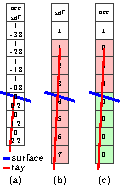
\includegraphics[width=1\linewidth]{fig/method_sdf_2}
    \end{subfigure}
    \hfill
    \begin{subfigure}[t]{0.5\linewidth}
        \vspace{3px}
        \centering
        \hspace*{-12px}
        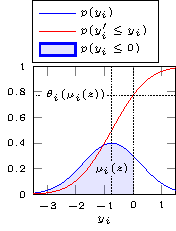
\includegraphics[width=1\linewidth]{fig/method_sdf_1}
    \end{subfigure}
    \vspace*{-10px}
    \caption{{\bf Left: Problem when Predicting SDFs.} Illustration of a ray ({\color{red}red}) correctly hitting a surface ({\color{blue}blue}) causing the SDF values and occupancy values in the underlying voxel grid to be correct (\cf (a)). A noisy ray, however, causes all voxels along the ray to get invalid distances assigned (marked {\colorbox{red!25}{red}}; \cf (b)). When using occupancy, in contrast, only the voxels behind the surface are assigned invalid occupancy states (marked {\colorbox{red!25}{red}}); the remaining voxels are labeled correctly (marked {\colorbox{green!25}{green}}; \cf (c)).
    {\bf Right: Proposed Gaussian-to-Bernoulli Transformation.} For $p(y_i) := p(y_i | z) = \mathcal{N}(y_i;\mu_i(z), \sigma^2)$ ({\color{blue}blue}), we illustrate the transformation discussed in Section \ref{subsec:method-inference}, allowing to use the binary observations $x_i$ (for $x_i \neq \uk$) to supervise the SDF predictions. This is achieved, by transforming the predicted Gaussian distribution to a Bernoulli distribution with occupancy probability $\theta_i(\mu_i(z)) = p(y_i \leq 0)$ ({\color{blue}blue area}).}
    \label{fig:method-sdf}
    \vspace*{-0.25cm}
\end{figure}

In order to still work with SDFs (to achieve sub-voxel accuracy) we propose to define $p(y_i = x_i | z)$ through a simple transformation. In particular, as $p(y_i | z)$ is modeled as Gaussian distribution $p(y_i | z) = \mathcal{N}(y_i ; \mu_i(z), \sigma^2)$ where $\mu_i(z)$ is predicted using the fixed decoder (and $\sigma^2 = 1$) and $x_i$ is binary (for $x_i \neq \uk$), we introduce a mapping $\theta_i(\mu_i(z))$ transforming the predicted Gaussian distribution to a Bernoulli distribution with occupancy probability $\theta_i(\mu_i(z))$, \ie, $p(y_i = x_i|z)$ becomes $\text{Ber}(y_i = x_i; \theta_i(\mu_i(z)))$.
%
%ag: no need to discuss this I think
%This is necessary, as the observation $x_i \neq \uk$ is inherently binary. Although we could derive distance functions from the observations, \eg, along the rays corresponding to observed points \ag{You had a paper here, right?}, even slight noise can result in large changes in the derived distances (along the whole ray). 
%
%\begin{align}
%p(y_i = x_i | z) = \text{Ber}(y_i = x_i; \theta_i(\mu_i(z)))
%\end{align}
As we defined occupied voxels to have negative sign in the SDF, we can derive the occupancy probability $\theta_i(\mu_i(z))$ as the probability of a negative distance:
\begin{align}
\theta_i(\mu_i(z)) &= \mathcal{N}(y_i \leq 0; \mu_i(z), \sigma^2)\label{eq:sdf}\\
%& = \int_{y_i'}^0 \mathcal{N}(y_i' \leq 0; \mu_i(z), \sigma^2) dy_i'\\
&= \frac{1}{2} \left(1 + \text{erf}\left(\frac{- \mu_i(z)}{\sigma \sqrt{\pi}}\right)\right).\label{eq:sdf-erf}
\end{align}
%
Here, $\text{erf}$ is the error function which, in practice, is approximated following \cite{Abramowitz1974}. Equation \eqref{eq:sdf} is illustrated in Figure~\ref{fig:method-sdf} where the occupancy probability $\theta_i(\mu_i(z))$ is computed as the area under the Gaussian bell curve for $y_i \leq 0$. This per-voxel transformation can easily be implemented as non-linearity layer and its derivative \wrt $\mu_i(z)$ is -- by construction -- a Gaussian distribution. Overall, this transformation allows to predict SDFs while using binary observations.